%!TEX TS-program = xelatex

% Шаблон документа LaTeX создан в 2018 году
% Алексеем Подчезерцевым
% В качестве исходных использованы шаблоны
% 	Данилом Фёдоровых (danil@fedorovykh.ru) 
%		https://www.writelatex.com/coursera/latex/5.2.2
%	LaTeX-шаблон для русской кандидатской диссертации и её автореферата.
%		https://github.com/AndreyAkinshin/Russian-Phd-LaTeX-Dissertation-Template

\documentclass[a4paper,14pt]{article}


%%% Работа с русским языком
\usepackage[english,russian]{babel}   %% загружает пакет многоязыковой вёрстки
\usepackage{fontspec}      %% подготавливает загрузку шрифтов Open Type, True Type и др.
\defaultfontfeatures{Ligatures={TeX},Renderer=Basic}  %% свойства шрифтов по умолчанию
\setmainfont[Ligatures={TeX,Historic}]{Times New Roman} %% задаёт основной шрифт документа
\setsansfont{Comic Sans MS}                    %% задаёт шрифт без засечек
\setmonofont{Courier New}
\usepackage{indentfirst}
\frenchspacing

\renewcommand{\epsilon}{\ensuremath{\varepsilon}}
\renewcommand{\phi}{\ensuremath{\varphi}}
\renewcommand{\kappa}{\ensuremath{\varkappa}}
\renewcommand{\le}{\ensuremath{\leqslant}}
\renewcommand{\leq}{\ensuremath{\leqslant}}
\renewcommand{\ge}{\ensuremath{\geqslant}}
\renewcommand{\geq}{\ensuremath{\geqslant}}
\renewcommand{\emptyset}{\varnothing}

%%% Дополнительная работа с математикой
\usepackage{amsmath,amsfonts,amssymb,amsthm,mathtools} % AMS
\usepackage{icomma} % "Умная" запятая: $0,2$ --- число, $0, 2$ --- перечисление

%% Номера формул
%\mathtoolsset{showonlyrefs=true} % Показывать номера только у тех формул, на которые есть \eqref{} в тексте.
%\usepackage{leqno} % Нумерация формул слева	

%% Перенос знаков в формулах (по Львовскому)
\newcommand*{\hm}[1]{#1\nobreak\discretionary{}
	{\hbox{$\mathsurround=0pt #1$}}{}}

%%% Работа с картинками
\usepackage{graphicx}  % Для вставки рисунков
\graphicspath{{images/}}  % папки с картинками
\setlength\fboxsep{3pt} % Отступ рамки \fbox{} от рисунка
\setlength\fboxrule{1pt} % Толщина линий рамки \fbox{}
\usepackage{wrapfig} % Обтекание рисунков текстом

%%% Работа с таблицами
\usepackage{array,tabularx,tabulary,booktabs} % Дополнительная работа с таблицами
\usepackage{longtable}  % Длинные таблицы
\usepackage{multirow} % Слияние строк в таблице
\usepackage{float}% http://ctan.org/pkg/float

%%% Программирование
\usepackage{etoolbox} % логические операторы


%%% Страница
\usepackage{extsizes} % Возможность сделать 14-й шрифт
\usepackage{geometry} % Простой способ задавать поля
\geometry{top=20mm}
\geometry{bottom=20mm}
\geometry{left=20mm}
\geometry{right=10mm}
%
%\usepackage{fancyhdr} % Колонтитулы
% 	\pagestyle{fancy}
%\renewcommand{\headrulewidth}{0pt}  % Толщина линейки, отчеркивающей верхний колонтитул
% 	\lfoot{Нижний левый}
% 	\rfoot{Нижний правый}
% 	\rhead{Верхний правый}
% 	\chead{Верхний в центре}
% 	\lhead{Верхний левый}
%	\cfoot{Нижний в центре} % По умолчанию здесь номер страницы

\usepackage{setspace} % Интерлиньяж
\onehalfspacing % Интерлиньяж 1.5
%\doublespacing % Интерлиньяж 2
%\singlespacing % Интерлиньяж 1

\usepackage{lastpage} % Узнать, сколько всего страниц в документе.

\usepackage{soul} % Модификаторы начертания

\usepackage{hyperref}
\usepackage[usenames,dvipsnames,svgnames,table,rgb]{xcolor}
\hypersetup{				% Гиперссылки
	unicode=true,           % русские буквы в раздела PDF
	pdftitle={Автоматизация проектных работ},   % Заголовок
	pdfauthor={Солодянкин А.А.},      % Автор
	pdfsubject={Автоматизация проектных работ},      % Тема
	pdfcreator={Солодянкин А.А.}, % Создатель
	pdfproducer={Солодянкин А.А.}, % Производитель
	pdfkeywords={Автоматизация проектных работ}, % Ключевые слова
	colorlinks=true,       	% false: ссылки в рамках; true: цветные ссылки
	linkcolor=black,          % внутренние ссылки
	citecolor=black,        % на библиографию
	filecolor=magenta,      % на файлы
	urlcolor=black           % на URL
}
\makeatletter 
\def\@biblabel#1{#1. } 
\makeatother
\usepackage{cite} % Работа с библиографией
%\usepackage[superscript]{cite} % Ссылки в верхних индексах
%\usepackage[nocompress]{cite} % 
\usepackage{csquotes} % Еще инструменты для ссылок

\usepackage{multicol} % Несколько колонок

\usepackage{tikz} % Работа с графикой
\usepackage{pgfplots}
\usepackage{pgfplotstable}

% ГОСТ заголовки
\usepackage[font=small]{caption}
%\captionsetup[table]{justification=centering, labelsep = newline} % Таблицы по правобу краю
%\captionsetup[figure]{justification=centering} % Картинки по центру


\newcommand{\tablecaption}[1]{\addtocounter{table}{1}\small \begin{flushright}\tablename \ \thetable\end{flushright}%	
\begin{center}#1\end{center}}

\newcommand{\imref}[1]{рис.~\ref{#1}}

\usepackage{multirow}
\usepackage{spreadtab}
\newcolumntype{K}[1]{@{}>{\centering\arraybackslash}p{#1cm}@{}}


\usepackage{xparse}
\usepackage{fancyvrb}

\RecustomVerbatimCommand{\VerbatimInput}{VerbatimInput}
{
	fontsize=\footnotesize    
}

\newcolumntype{?}[1]{!{\vrule width #1}}

\usepackage{tocloft}
\renewcommand{\cftsecleader}{\cftdotfill{\cftdotsep}}
\begin{document} % конец преамбулы, начало документа
\begin{titlepage}
	\begin{center}
		ПРАВИТЕЛЬСТВО РОССИЙСКОЙ ФЕДЕРАЦИИ \\
 		ФЕДЕРАЛЬНОЕ  ГОСУДАРСТВЕННОЕ АВТОНОМНОЕ \\
		ОБРАЗОВАТЕЛЬНОЕ УЧРЕЖДЕНИЕ ВЫСШЕГО ОБРАЗОВАНИЯ\\
		«НАЦИОНАЛЬНЫЙ ИССЛЕДОВАТЕЛЬСКИЙ УНИВЕРСИТЕТ\\
		«ВЫСШАЯ ШКОЛА ЭКОНОМИКИ»
	\end{center}
	
	\begin{center}
		\textbf{Московский институт электроники и математики}
		
		\textbf{Им. А.Н.Тихонова НИУ ВШЭ}
		
		\vspace{2ex}
		
		\textbf{Департамент компьютерной инженерии}
	\end{center}
	\vspace{1ex}	
	
	\vspace{1ex}
	\begin{center}
		\textbf{Практическая работа №7 \\
			<<Математические модели для решения задач размещения на печатной плате>> \\
			по курсу <<Автоматизация проектных работ>>\\
	}
	\end{center}	

	\vspace{2ex}
	\vfill
	
	\vspace{2ex}
	
	\begin{flushright}
		\textbf{Выполнил:}
		
		\vspace{2ex}
		
		Студент группы БИВ174
		
		\vspace{2ex}
		
		Солодянкин Андрей Александрович
		
		\vspace{2ex}
		
		\textbf{Проверил:}
		
		\vspace{2ex}
		
		Новиков Константин Викторович
	\end{flushright}

	\vspace{5ex}
	\begin{center}
		Москва \the\year \, г.
	\end{center}
	
\end{titlepage}
\addtocounter{page}{1}
\tableofcontents
\pagebreak

\section{Задание}

Провести моделирование с использованием ПО амплитудно-частотных и временных характеристик колебательного контура. Определить погрешность расчета временных характеристик при значениях сопротивления 10 и 100 Ом.

\section{Краткие теоретические сведения}

Колебательный контур -- осциллятор, представляющий собой электрическую цепь, содержащую соединённые катушку индуктивности и конденсатор. 
В такой цепи могут возбуждаться колебания тока (и напряжения).

Колебательный контур -- простейшая система, в которой могут происходить свободные электромагнитные колебания.
Резонансная частота контура определяется так называемой формулой Томсона:

\begin{equation}
f_0 = \frac{1}{2 \pi \sqrt{LC}}
\end{equation}

Принцип действия:
Пусть конденсатор ёмкостью C заряжен до напряжения $U_0$. 
Энергия, запасённая в конденсаторе составляет $E_c = \frac{C U_0^2}{2} $

При соединении конденсатора с катушкой индуктивности, в цепи потечёт ток, что вызовет в катушке электродвижущую силу (ЭДС) самоиндукции, направленную на уменьшение тока в цепи. 
Ток, вызванный этой ЭДС (при отсутствии потерь в индуктивности) в начальный момент будет равен току разряда конденсатора, то есть результирующий ток будет равен нулю. 
Магнитная энергия катушки в этот (начальный) момент равна нулю.

Затем результирующий ток в цепи будет возрастать, а энергия из конденсатора будет переходить в катушку до полного разряда конденсатора. 
Магнитная же энергия, сосредоточенная в катушке, напротив, максимальна и равна $E_L = \frac{L I_0^2}{2} $, где $L$ -- индуктивность катушки, $I_0$ максимальное значение тока.

После этого начнётся перезарядка конденсатора, то есть заряд конденсатора напряжением другой полярности.
Перезарядка будет проходить до тех пор, пока магнитная энергия катушки не перейдёт в электрическую энергию конденсатора.
Конденсатор, в этом случае, снова будет заряжен до напряжения $U$.

В результате в цепи возникают колебания, длительность которых будет обратно пропорциональна потерям энергии в контуре.

В общем, описанные выше процессы в параллельном колебательном контуре называются резонанс токов, что означает, что через индуктивность и ёмкость протекают токи, больше тока проходящего через весь контур, причем эти токи больше в определённое число раз, которое называется добротностью. 
Эти большие токи не покидают пределов контура, так как они противофазны и сами себя компенсируют. 
Стоит также заметить, что сопротивление параллельного колебательного контура на резонансной частоте стремится к бесконечности (в отличие от последовательного колебательного контура, сопротивление которого на резонансной частоте стремится к нулю), а это делает его незаменимым фильтром.

Стоит заметить, что помимо простого колебательного контура, есть ещё колебательные контуры первого, второго и третьего рода, что учитывают потери и имеют другие особенности.

Амплитудно-частотная характеристика (АЧХ) -- зависимость амплитуды выходного сигнала от частоты.
А также функция выражающая (описывающая) эту зависимость. 
А также -- график этой функции. 
Математически амплитуда -- это модуль некоторой комплекснозначной функции от частоты.
Также может рассматриваться АЧХ других комплекснозначных функций частоты, например, спектральной плотности мощности сигнала.

АЧХ в теории линейных стационарных систем означает зависимость модуля передаточной функции системы от частоты.
АЧХ показывает во сколько раз амплитуда сигнала на выходе системы отличается от амплитуды входного сигнала на всём диапазоне частот.

На графике АЧХ по оси абсцисс откладывается частота, а по оси ординат отношение амплитуд выходного и входного сигналов системы. 
Обычно для частоты используется логарифмический масштаб, так как исследуемый диапазон частот может изменяться в достаточно широких пределах (от единиц до миллионов Гц или рад/с). 
В случае когда логарифмический масштаб используется и на оси ординат, АЧХ превращается в логарифмическую амплитудно-частотную характеристику. 
ЛАЧХ получила широкое распространение в теории автоматического управления в связи с простотой построения и наглядностью при исследовании систем управления.

\section{Выполнение работы}

\begin{figure}[H]
	\centering
	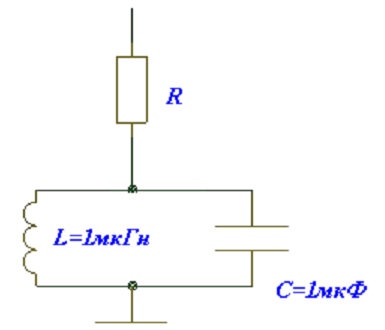
\includegraphics[width=0.4\linewidth]{image/schema}
	\caption{Схема колебательного контура}
	\label{fig:schema}
\end{figure}

\subsection{АЧХ}

АЧХ колебательного контура для сопротивлений 1, 10 и 100 Ом изображены на рис.~\ref{fig:afr_1}-\ref{fig:afr_100}.

\begin{figure}[H]
	\centering
	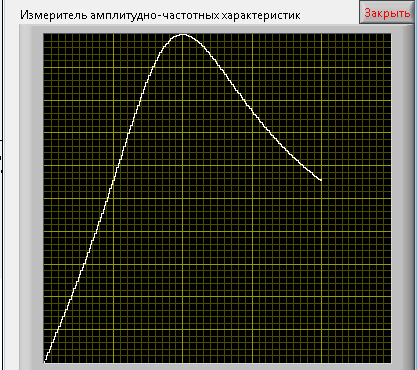
\includegraphics[width=0.5\linewidth]{image/afr_1}
	\caption{Амплитудно-частотная характеристика при R=1Ом}
	\label{fig:afr_1}
\end{figure}

\begin{figure}[H]
	\centering
	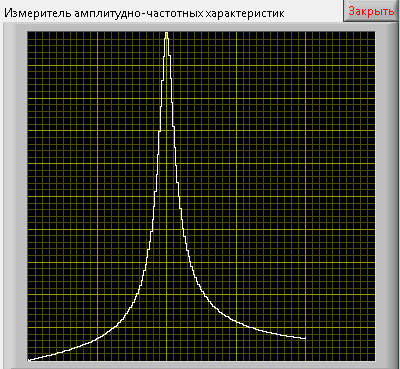
\includegraphics[width=0.5\linewidth]{image/afr_10}
	\caption{Амплитудно-частотная характеристика при R=10Ом}
	\label{fig:afr_10}
\end{figure}

\begin{figure}[H]
	\centering
	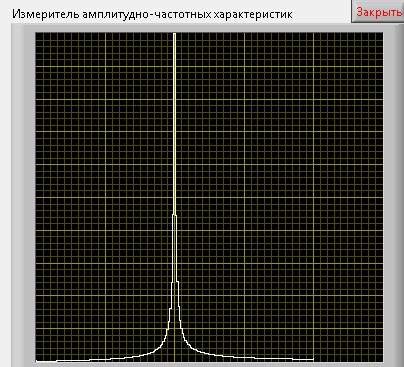
\includegraphics[width=0.5\linewidth]{image/afr_100}
	\caption{Амплитудно-частотная характеристика при R=100Ом}
	\label{fig:afr_100}
\end{figure}

\subsection{Временная характеристика}

Временная характеристика колебательного контура для различных значений сопротивлений при амплитуде сигнала $U_{in} = 1V$ и частотой $F_0=159kHz$ изображены на рис.~\ref{fig:time_1}-\ref{fig:time_100}.

\begin{figure}[H]
	\centering
	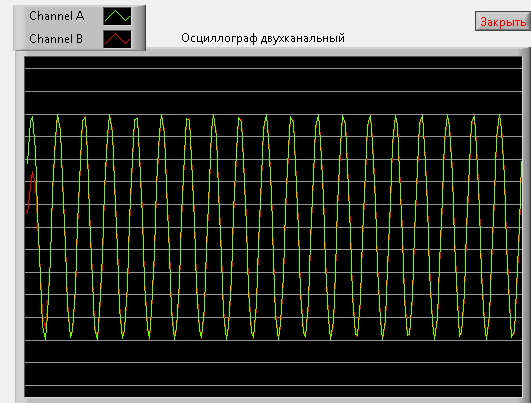
\includegraphics[width=0.5\linewidth]{image/time_1}
	\caption{Временная характеристика при R=1Ом}
	\label{fig:time_1}
\end{figure}

\begin{figure}[H]
	\centering
	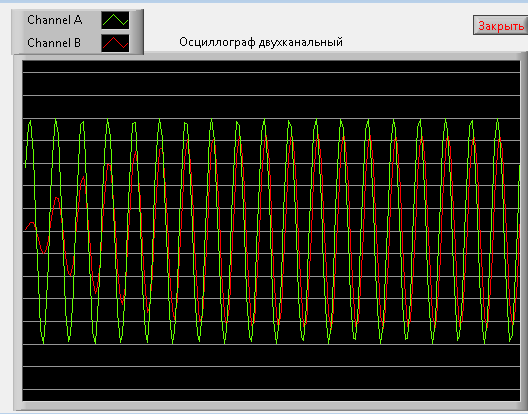
\includegraphics[width=0.5\linewidth]{image/time_10}
	\caption{Временная характеристика при R=10Ом}
	\label{fig:time_10}
\end{figure}

\begin{figure}[H]
	\centering
	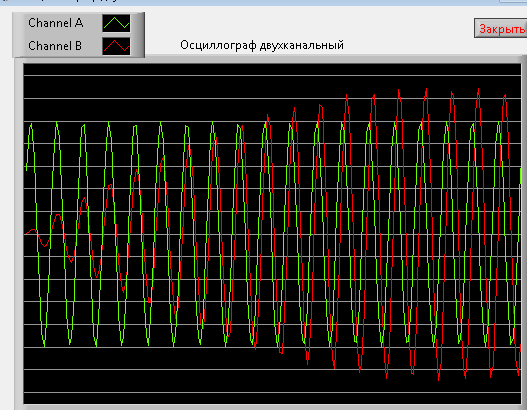
\includegraphics[width=0.5\linewidth]{image/time_100}
	\caption{Временная характеристика при R=100Ом}
	\label{fig:time_100}
\end{figure}

\begin{table}[H]
	\begin{center}
		\begin{flushleft}
			\tablecaption{Зависимость выходного напряжения от сопротивления}
		\end{flushleft}
		\label{tab:task_1}
		\begin{tabular}{|c|c|}
			\hline
			$R$, Ом & $U_{out}$, В \\ \hline
			1       & 0,998024     \\ \hline
			10      & 0,864529     \\ \hline
			100     & 0,258269     \\ \hline
		\end{tabular}
	\end{center}
\end{table}

\subsection{Погрешность}

Погрешность временных характеристик осуществляется по формуле:

\begin{equation}
\frac{U_{in} - U_{out}}{U_{in}}
\end{equation}

Для R = 10 Ом погрешность составляет 0,135В.

Для R = 100 Ом погрешность составляет 0,742В.

\section{Выводы по работе}


В	результате выполнения лабораторной были рассчитаны амплитудно-частотные и временные характеристики колебательного контура при различных значениях сопротивления. На основе результатов была рассчитана погрешность.


\section{Контрольные вопросы}

\begin{enumerate}
	\item Математическая модель схемы во временной области и методы ее расчета.
	
	Математическая модель схемы во временной области имеет вид: 
	\begin{equation}
	I(V', V, t) = 0
	\end{equation}
	\begin{itemize}
		\item $I$ - нелинейная вектор-функция, представляющая собой алгебраическую сумму токов в узле;
		
		\item $V'$ - вектор производных узловых потенциалов по времени;
		
		\item $V$ - вектор узловых потенциалов;
		
		\item $t$ - время. 
	\end{itemize}


	В подсистемах схемотехнического анализа применяются методы, основанные:
	\begin{itemize}
		\item на формулах дифференцирования назад (ФДН),
		\item на циклическом применении неявной и явной формул Эйлера (циклический алгоритм). 
	\end{itemize}
	
	\item Объясните, чем вызвано увеличение погрешности расчета временных характеристик при увеличении R.
	
	При увеличении сопротивления, токи уменьшаются, конденсатор  дольше заряжается, дольше устанавливается стационарный режим работы, а так же увеличивается погрешность.
\end{enumerate}

\end{document} % конец документа